
\subsection{Annihilation}

When a particle meets its antiparticle, the particles annihilate.  They cease to exist, and in their place {\bf two}\footnote{Two photons are needed in order to conserve both energy and momentum.} photons are created, of gamma ray energies.  The mass of the particles is converted into the energy of the gamma rays, according to the equivalence between mass and energy given by the formula $E=mc^{2}$.

\begin{marginfigure}
\begin{tikzpicture}[thick]
\draw[->]  (-0.5,0.5) node[anchor=south] {\APelectron} --(-0.1,0.1); 
\draw[->]  (0.5,-0.5) node[anchor=north] {\Pelectron} --(0.1,-0.1);
\draw[fill=black] (0.5,-0.5) circle (0.075) ;
\draw[fill=black] (-0.5,0.5) circle (0.075) ;
\draw[decorate,decoration={snake}] (0.4,0.4)--(1.4,1.4);
\draw[->](1.4,1.4)--(1.5,1.5)node[anchor=south]{\Pphoton};
\draw[decorate,decoration={snake}] (-0.4,-0.4)--(-1.4,-1.4);
\draw[->](-1.4,-1.4)--(-1.5,-1.5)node[anchor=north]{\Pphoton};
\begin{scope}[thin]
\node [star, star points=10, star point height=.2cm, minimum size=1cm, draw]
at (0,0) {};
\end{scope}
\end{tikzpicture}
\caption{A conceptual diagram (not to scale nor to be taken too literally!) to show the annihilation of an electron and its antiparticle the positron.  Two gamma ray photons, each having energy \SI{511}{keV}, are emitted in opposite directions.}
\end{marginfigure}

Consider the annihilation of an electron and a positron.  Presuming that almost all of their energy is that due to their masses (this is reasonable when their speed is small compared to the speed of light, since then their rest mass energy is likely to be much larger than their kinetic energy), the energy they together contain due to their masses is given by $E=mc^{2}=2m_{\mathrm{e}}c^{2}$, where $m_{\mathrm{e}}$ is the rest mass of an electron.  The total energy of the two photons produced must be equal to this amount of energy $2m_{\mathrm{e}}c^{2}$, due to the law of conservation of energy. Since this is shared equally between two photons, each of these has energy $m_{\mathrm{e}}c^{2}$.  This allows the frequency of the gamma ray photons to be identified (using $E=hf$), which can give an indication of what kind of particles annihilated.

\subsection{Pair production}

A sufficiently energetic photon of electromagnetic radiation can interact with an atomic nucleus (or some other object like an electron) and thereby create a particle--antiparticle pair.

\begin{figure}
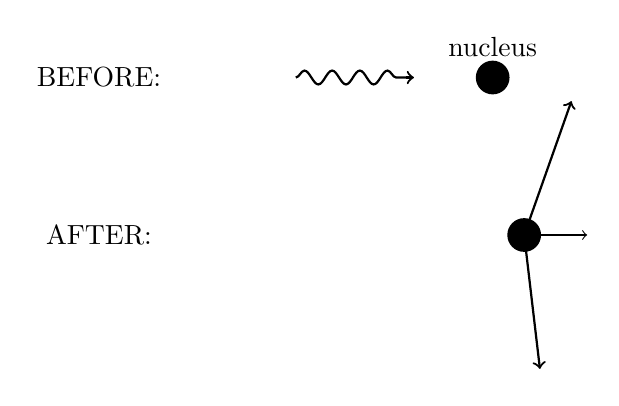
\begin{tikzpicture}[thick]
\draw (-2,0) node  {BEFORE:};
\draw (-2,-2) node {AFTER:};
\draw[fill=black] (3,0) circle (0.2) node[above=4pt]{nucleus};
\draw[decorate,decoration={snake}] (0.5,0)node[anchor=east]{\Pphoton}--(1.9,0);
\draw[->] (1.9,0)--(2.0,0);
\draw[fill=black]  (3,-2) ++(0.4,0) circle (0.2);
\begin{scope}[thin]
\draw[->](3,-2) ++(0.4,0)--++(0.8,0);
\end{scope}
\draw[->](3.4,-2) ++(0,0)--++(0.2+0.4,1.7)node[anchor=west]{\Pelectron};
\draw[->](3.4,-2) ++(0,0)--++(-0.2+0.4,-1.7)node[anchor=west]{\APelectron};
\end{tikzpicture}
\caption{A conceptual diagram showing a pair production process (in this case, an electron--positron pair is produced).  The incoming photon has to interact with another body e.g.\ a nucleus, in order to conserve both energy and momentum; the nucleus or electron recoils (consider the time-reversal of this process in the zero-momentum frame to see this).}
\end{figure}

Commonly, electron--positron pairs are produced,\footnote{In detectors---the positron was first discovered in a cloud chamber by Carl Anderson in 1932---a magnetic field is applied, and this means that pair production of charged particles can be easily seen as the pair curve away in opposite directions due to their opposite charges.} as these are relatively light and so the energy of the incoming photon does not have to be too high.  In order to produce an electon--positron pair, the incoming photon must have enough energy to produce the total mass, which is $2m_{\mathrm{e}}c^{2}$, so the minimum energy of the photon must be $E=hf=2m_{\mathrm{e}}c^{2}$.  Any excess energy of the photon goes into kinetic energy of the electron and positron.
